%
%  hume.five
%
%  Created by Mark Eli Kalderon on 2007-08-04.
%  Copyright (c) 2007 Mark Eli Kalderon. All rights reserved.
%
%  Beamer

% Definitions and macros
\newcommand{\change}{\textcolor{blue}{\textbf{CHANGE SLIDE}}}
\def\myauthor{Mark Eli Kalderon} 
\def\mytitle{Introduction to Moral Philosophy}
\def\mysubtitle{Hume}
\def\myinstitution{University College London}
\def\myurl{http://markelikalderon.com}

% Packages specific to lecture notes
\mode<article>{
    \usepackage{palatino}
}

% Packages specific to beamer presentation
\mode<presentation>{
    \usetheme{Darmstadt}
    \setbeamercovered{transparent}
    \pgfdeclareimage[height=0.5cm]{university-logo}{../../../graphics/logo_sml_blk}
    \logo{\pgfuseimage{university-logo}}
}

% Packages common to lecture notes and beamer presentation
\usepackage{pgf}
\usepackage{tikz}
\usepackage{hyperref}

\setjobnamebeamerversion{hume.five.beamer}

\title{\mytitle}
\subtitle{\mysubtitle}

\author{\myauthor\\
\url{\myurl}}
\institute{\myinstitution}

\hyphenation{ap-pro-ba-tion}

% \date[Short Occasion] % (optional)
% {Date / Occasion}

\begin{document}

\frame{\maketitle}

\section{Main Points from Last Time}\label{sec:main_points_from_last_time} % (fold)

\change\ Last time we completed Hume's argument in favor of moral sentimentalism over moral rationalism. The traditional debate between moral rationalists and moral sentimentalists concerned whether it was by means of reason or internal sentiment that we distinguish between vice and virtue. In Hume's framework, this becomes the question whether it is by means of the relations among ideas or by impressions that we distinguish between vice and virtue. Moral rationalism, so conceived faced two basic problems. First, moral judgments influence the will; but it is hard to understand how knowledge of relations would necessarily determine the will. Second, the relations had to obtain between perceptions in the mind and external objects if they are to determine the vice and virtue of actions, sentiments, and characters, but it is hard to conceive of any relevant relation that would not also hold of perceptions alone or of external objects alone; but if that's right, moral rationalism overgenerates---it counts as virtuous or visious things that could not be. For these reasons Hume favors moral sentimentalism over moral rationalism. 

Hume thus maintains that the distinction between vice and virtue is determined by impressions, specifically by passions or internal sentiment. Specifically, Hume maintains that moral distinctions just are particular pains or pleasures occassioned upon the general view or survey. Virtue and vice involve aggreable and disagreeable impressions. Moreover these agreeable and disagreeable impressions are peculiar to their objects. Moral pleasures and pains are a distinctive kind of pleasure and pain that differs in kind from, say, the pleasure we take in a good bottle of wine or in a roast hog. 

\change\ Since moral distinctions just are particular pains or pleasures occasioned upon the general view or survey, to explain our distinctions between virtue and vice it suffices to explain the circumstances that occasion moral approbation and disapprobation. Are the principles that explain moral pleasures and pains natural? According to Hume, this question has no straightforward answer since distinct senses of ``natural'' can be distinguished:

\begin{itemize}
    \item In one sense, natural contrasts with \emph{miraculous}. Not only is the distinction between virtue and vice natural in this sense, but so is everything else ``\emph{excepting those miracles, on which our religion is founded}'' (\emph{Treatise}, 3.1.2.7).
    \item In another sense, natural contrasts with \emph{unusual}. The distinction between virtue and vice is natural in this sense. Hume observes that there never was a nation in the world nor a single person in any nation, who was utterly lacking in the moral sense (\emph{Treatise}, 3.1.2.8).
    \item In another sense, natural contrasts with \emph{artificial}. It is important to recognize the intended contrast. Natural, here, is not being contrasted with the unreal or fake, but rather with what is the product of human artifice. Hume claims that while certain virtues such as benevolence are natural, other virtues such as justice are artificial. While the moral approbation we feel towards benevolent acts is natural, the moral approbation we feel towards just acts is partly the result of artifice and human convention.
\end{itemize}

Natural virtues include benevolence, generosity, charity, love of life, and kindness to children. Artificial virtues include justice, fidelity, honesty, and chastity. \change

Natural virtues have two important features:

\begin{enumerate}
	\item First, natural virtues are implanted instincts. They involve behavioral dispositions native to human beings. More specifically, they involve natural dispositions to perform certain types of actions under certain types of circumstances. So, for example, the natural virtue of kindness to children involves the disposition to feed a child if the child is hungry.
    \item Second, the manifestation of natural virtue invariably results in good. Each performance of the relevant type of action in the relevant type of circumstance results in some good. So for example, when kindness moves us to feed a hungry child, this action results in some good---the hunger of the child is abated.
\end{enumerate}

In contrast, the artificial virtues differ in both these respects from the natural virtues:

\begin{enumerate}
	\item First, the artificial virtues are not implanted instincts. Rather the artificial virtues involve dispositions to behave in accordance with a general scheme or convention, itself a product of human artifice. Observances of the general scheme are too various and complex for each to be the result of a distinct behavioral disposition native to human beings.
    \item Second, the manifestation of artificial virtue does not invariably result in good. It is not the case that every observance of the general scheme benefits either the private individual or the public. Justice, for example, may require us to repay a debt to an enemy or to someone who will use the funds to some malicious end contrary to the public good. It is the general compliance with the scheme or convention that benefits the public and not any particular observance of that general scheme.
\end{enumerate}

Justice is Hume's central example of an artificial virtue. In the first section of part two, Hume establishes his main negative conclusion: Hume argues that justice could not be a natural virtue. In the second section of part two, Hume gives his positive account of justice as an artificial virtue.
Hume's positive account has two stages. The first stage is a genealogy of justice: Hume explains the motives and circumstances that first established the conventions of justice. The second stage is an account of the moral beauty of just acts: Hume gives a separate explanation for why observances of these conventions have merit and are the proper object of moral approbation. Notice that the original motive to justice is not the principle that bestows merit upon just acts, that is, particular observances of the general scheme.
This is an important further difference between natural and artificial virtues. With respect to the natural virtues, the motive to virtuous action is what bestows merit upon that action. Consider kindness to children. When you feed a hungry child, the motive is kindness, and it is the amiableness of this action, its being motivated by kindness, that bestows merit upon the action and makes it the object of moral approbation. With artificial virtues, however, the original motive for virtuous action is distinct from the principle that bestows merit upon the action and makes it the object of moral approbation. \change

% \textbf{See Figure~\ref{fig:slide1}.}
% 
% \begin{figure}[ht]
%     \begin{center}
%         \includeslide[height=5cm]{slide1<1>}
%     \end{center}
%     \caption{Main Points from Last Time}
%     \label{fig:slide1}
% \end{figure}

\frame<presentation>[label=slide1]{
    \frametitle{Main Points From Last Time}
        \begin{columns}
            \begin{column}{3cm}
                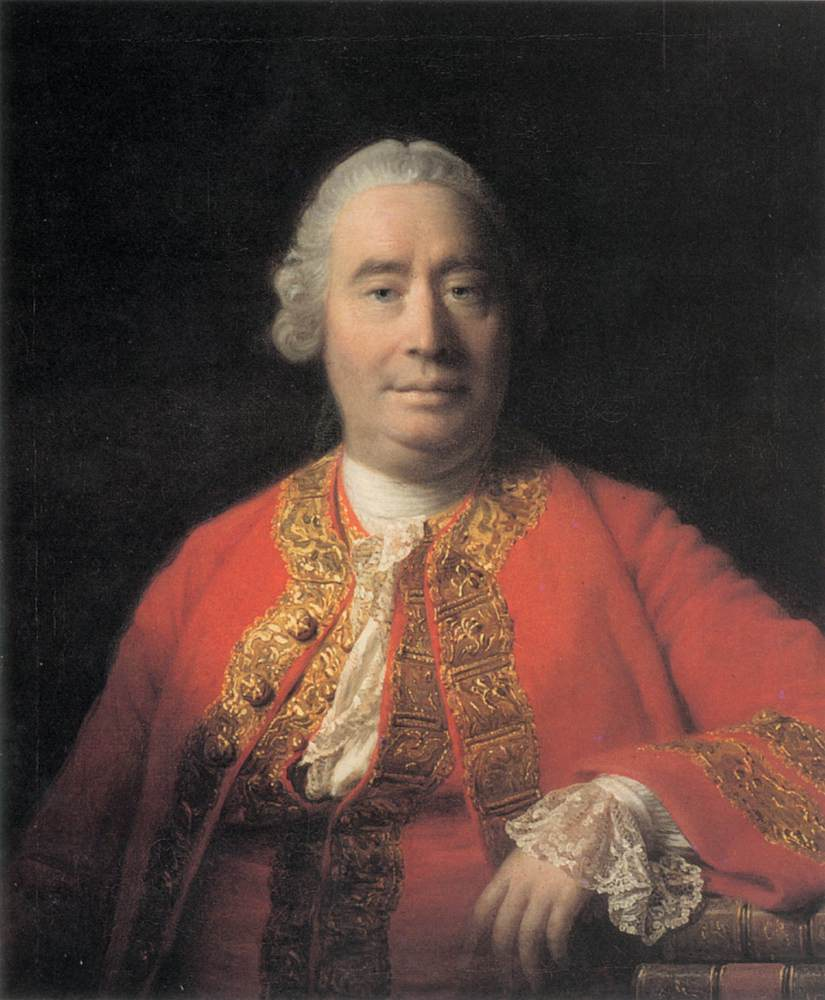
\includegraphics[height=4cm]{../../../graphics/hume.jpg}
            \end{column}
            \begin{column}{7cm}
                \begin{itemize}
                    \item<1-> Moral distinctions are particular pleasures or pains occasioned upon the general view or survey
                    \item<2-> Are moral distinctions natural? Depends on in what sense
                    \item<3-> Whereas, \alert{natural virtues} are implanted instincts whose manifestation invariably results in some good; \alert{artificial virtues} are not implanted instincts, they are dispositions to behave in accordance with convention and their manifestations do not invariably result in some good
                \end{itemize}
            \end{column}
        \end{columns}
}

% section main_points_from_last_time (end)

\section{Why Justice is Not a Natural Virtue}\label{sec:why_justice_is_not_a_natural_virtue} % (fold)

Let’s begin with Hume’s negative case. Why does Hume deny that justice is a natural virtue? \emph{Treatise} 3.2.1 is dedicated to establishing Hume’s negative case.

The overall structure of Hume's argument is relatively clear---even though, as we will see, it is controversial how to interpret crucial transitions of that argument. The argument can be outlined as follows:

\begin{enumerate}
    \item All virtuous actions derive their merit only from virtuous motives. (\emph{Treatise}, 3.2.1.2-4)
    \item The virtuous motive could not be the ``regard to the virtue'' of the action, a sense of duty, since this involves a vicious circularity. (Treatise, 3.2.1.4-8)
    \item So there must be an independent motive, distinct from the sense of duty, for any virtuous action. What independent motive could there be for just action? (\emph{Treatise}, 3.2.1.9)
    \item If we restrict ourselves to natural affections (motives available in the rude and natural state of humankind) such as self-love and public and private benevolence, no motive sufficient to the establishment of justice can be found. (\emph{Treatise}, 3.2.1.10-16)
    \item So there could be no motive to just action independent of a regard to the justice of that action, a sense of duty. (Treatise, 3.2.1.17)
    \item Unless, ``nature has establish'd a sophistry'' the solution to this paradox, is that the sense of justice does not derive from nature but from artifice---that justice is not a natural virtue but an artificial virtue. (\emph{Treatise}, 3.2.1.17)
\end{enumerate}

It is not yet clear how to interpret the reasoning in the final stage of the argument, but it does suggest that the argument is supposed to be a \emph{reductio ad absurdum} of the claim that justice is a natural virtue.

Before we can understand the \emph{reductio}, we must first understand the nature of the circularity introduced in the second stage of the argument. The claim that justice is a natural virtue is reduced to absurdity, in part due to the incoherence of reasoning in a circle. So we need to try and understand how the circularity in the second stage of Hume's argument can give rise to an incoherence sufficient to underwrite the \emph{reductio}.

But before we can understand how the circle might be incoherent, we must first understand Hume's claim that all virtuous actions derive their merit from virtuous motives---for it plays a crucial role in generating the circle. \change

% \textbf{See Figure~\ref{fig:slide2}.}
% 
% \begin{figure}[ht]
%     \begin{center}
%         \includeslide[height=5cm]{slide2<1>}
%     \end{center}
%     \caption{Justice is Not an Artificial Virtue}
%     \label{fig:slide2}
% \end{figure}

\frame<presentation>[label=slide2]{
    \frametitle{Justice is Not an Artificial Virtue}
        \alert{P1} All virtuous actions derive their merit only from virtuous motives.\\
        \alert{P2} The virtuous motive could not be the ``regard to the virtue'' of the action, a sense of duty, since this involves a vicious circularity.\\
        \alert{P3} So there must be an independent motive, distinct from the sense of duty, for any virtuous action.\\
        \alert{P4} If we restrict ourselves to natural affections (motives available in the rude and natural state of humankind) such as self-love and public and private benevolence, no motive sufficient to the establishment of justice can be found.\\
        \alert{P5} So there could be no motive to just action independent of a regard to the justice of that action, a sense of duty.\\
        \alert{C} So, unless, ``nature has establish'd a sophistry'', justice must be an artificial virtue.
}

% section why_justice_is_not_a_natural_virtue (end)

\subsection{Virtuous Actions \& Virtuous Motives}\label{sec:virtuous_actions_and_virtuous_motives} % (fold)

We have seen that, for Hume, the objects of moral evaluation are actions, sentiments, and characters. In \emph{Treatise} 3.2.1, Hume importantly qualifies this claim. Actions may be judged virtuous or vicious but only \emph{derivatively}---an action is virtuous or vicious only if its motive is virtuous or vicious. Later in the \emph{Treatise}, Hume will qualify this doctrine further---it is relatively stable configurations of passions and sentiments---characters, that are the primary objects of moral evaluation. It is this feature of Hume's ethics that makes it a \emph{virtue theory}, placing Hume in a tradition that includes Aristotle before him and Nietzsche after him.

An action may have merit---it may be the genuine object of moral approbation---but only when considered as a sign for the motive that produced it. It is the motive that is the primary object of moral approbation, and it is the motive that primarily has merit. An action considered by itself, independently of its motive, lacks merit in the radical sense of not being a candidate for moral evaluation:

\begin{quote}
    The external performance has no merit. We must look within to find the moral quality. This we cannot do directly; and therefore fix our attention on actions, as on external signs. but these actions are still consider'd as signs; and the ultimate object of our praise and approbation is the motive, that produc'd them. (\emph{Treatise}, 3.2.1.2)
\end{quote}

Not only is the motive the primary object of moral approbation when we praise a person for acting as virtue requires, but it is also the primary object of moral disapprobation when we blame a person for not acting as virtue requires. We blame a person who does not act virtuously for not being moved by the relevant virtuous motive. So when malice moves a man to give a hungry child a stone instead of bread, he displays a want of natural affection for the child and so is blameable on that account. Contrast this with cases where the virtuous motive is present ``tho' check'd in its operation by some circumstances unknown to us''. In such cases, we do not blame the person for not acting as virtue requires. It is the person's motivation and not their action that is the primary object of moral disapprobation.

So far, these are claims about the objects of moral approbation and disapprobation. They answer the questions:
\begin{itemize}
    \item What are the objects of moral approbation and disapprobation?
    \item What has merit or demerit?
\end{itemize}
It is actions produced by certain motives that are the objects of moral approbation and disapprobation. But there are other questions that a moral scientist might naturally ask:
\begin{itemize}
    \item What makes it the case that something is the object of moral approbation and disapprobation?
    \item What bestows merit or demerit upon something?
\end{itemize}
Having established that an action has merit and is the object of moral approbation only when considered as a sign for the motive that produced it, a moral scientist might seek an explanation for this. A natural hypothesis immediately suggests itself: It is the motive that produced the action that bestows merit upon the action and makes it the object of moral approbation. Hume describes the hypothesis this way:
\begin{quote}
    It appears, therefore, that all virtuous actions derive their merit only from virtuous motives, and are consider’d merely as signs for these motives. (Treatise, 3.2.1.4)
\end{quote}
Virtuous actions derive their merit from the motives that produce them in the sense that these motives bestow merit upon those actions and makes them the proper objects of moral approbation. This is an important further claim. It is one thing for actions produced by certain motives to be the objects of moral approbation, it is another thing for these actions to be the objects of moral approbation because of the motives that produced them. \change

% \textbf{See Figure~\ref{fig:slide3}.}
% 
% \begin{figure}[ht]
%     \begin{center}
%         \includeslide[height=5cm]{slide3<1>}
%     \end{center}
%     \caption{Virtuous Action \& Virtuous Motive}
%     \label{fig:slide3}
% \end{figure}

\frame<presentation>[label=slide3]{
    \frametitle{Virtuous Action \& Virtuous Motive}
        \begin{columns}
            \begin{column}{3cm}
                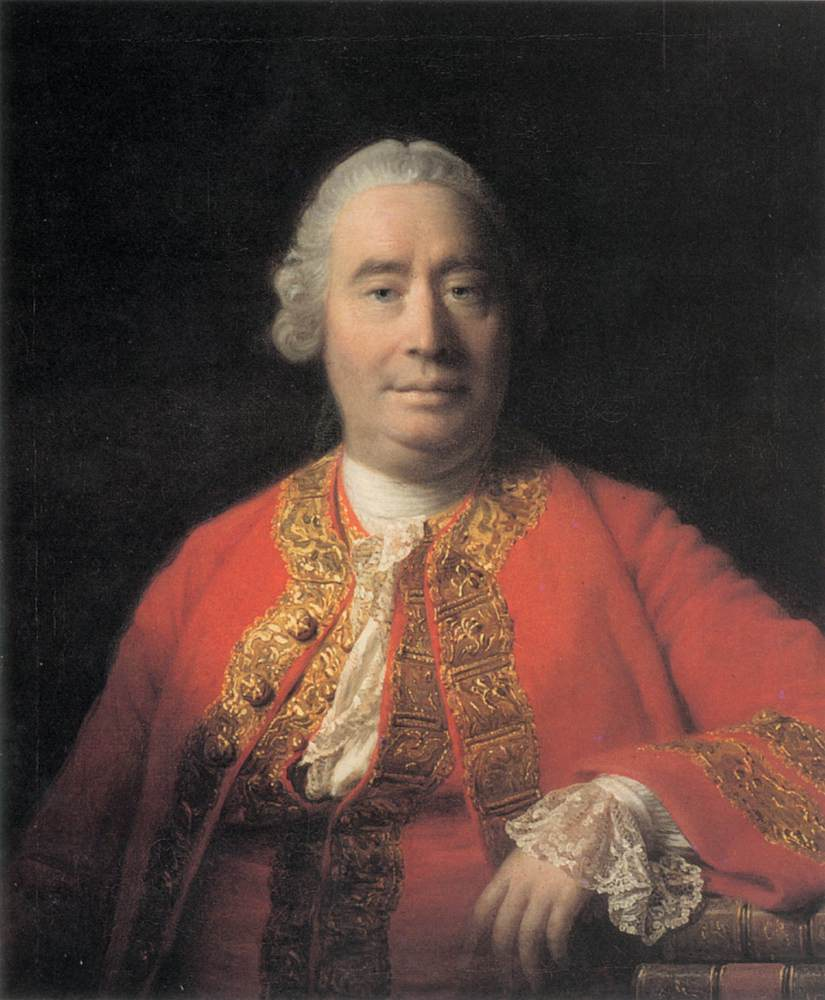
\includegraphics[height=4cm]{../../../graphics/hume.jpg}
            \end{column}
            \begin{column}{7cm}
                ``The external performance has no merit. We must look within to find the moral quality.'' (\emph{Treatise}, 3.2.1.2)\\
                ``\ldots all virtuous actions derive their merit only from virtuous motives, and are consider'd merely as signs of these motives.'' (\emph{Treatise}, 3.2.1.4)
            \end{column}
        \end{columns}
}

% section virtuous_actions_and_virtuous_motives (end)

\subsection{The Circle}\label{sec:the_circle} % (fold)

This explanatory hypothesis has important consequences. From it Hume concludes that ``the first virtuous motive, which bestows a merit on any action, can never be a regard to the virtue of that action, but must be some other natural motive or principle'':
\begin{quote}
    To suppose, that the mere regard to the virtue of the action, may be the first motive, which produc’d the action, and render’d it virtuous, is to reason in a circle. Before we can have such a regard, the action must be really virtuous; and this virtue must be deriv’d from some virtuous motive: And consequently the virtuous motive must be different from the regard to the virtue of the action. A virtuous motive is requisite to render an action virtuous. An action must be virtuous, before we can have a regard to its virtue. Some virtuous motive, therefore, must be antecedent to that regard. (\emph{Treatise}, 3.2.1.4)
\end{quote}

If an action derives its merit from the motive that produced it, the motive that produces a virtuous action and bestows merit upon it could not be a regard to its virtue, for an action must already have merit before we can have a regard to its virtue.

At first blush, Hume’s reasoning here is relatively clear. However, the precise sense in which one would be reasoning in a circle and why it would be vicious has eluded commentators. There is no consensus on how to interpret Hume here, and many doubt that Hume has a coherent position. I can only sketch the difficulties as I understand them; we will return to the question of how Hume might be charitably interpreted.

``What makes an action virtuous?'', Hume asks. For the sake of concreteness, let’s consider a candidate virtuous action, repaying a debt owed to a creditor. \change

In asking what makes an action virtuous, we might be asking:
\begin{itemize}
    \item In what does the merit of repaying a debt consist? 
    \item Why is repaying a debt the object of moral approbation?
\end{itemize}
These are the kind of questions that Hume’s explanatory hypothesis is supposed to answer. Repaying a debt has merit and is the object of moral approbation because of its motivation. It is the action’s motivation that bestows merit upon it. \change

However there is another kind of question that might be being asked. Recall that, for Hume, an action is only virtuous if it proceeds from a virtuous motive. So if an action lacks a virtuous motive, that action is not virtuous even if it is the same type of action as a genuinely virtuous action. Since the same type of action can proceed from different motives, and this can make a difference to the moral evaluation of the action, one might ask of an action of a given type, what makes it virtuous? If actions of the same type can vary in their virtue, how are we to distinguish genuinely virtuous actions from actions that merely appear to be virtuous? This gives us our second sense of the question. In asking what makes an action virtuous Hume might be asking:
\begin{itemize}
    \item What makes repaying a debt genuinely virtuous? 
    \item Which repayments are the objects of moral approbation?
\end{itemize}
These are questions about the objects of moral approbation.

Not only are these questions conceptually distinct, but they also seem to admit of distinct answers. Consider the regard to the virtue of an action. In acting out of regard for the virtue of the action, a person acts out of a general and nonspecific sense of duty, out of a motive to do whatever virtue requires. A motive to perform whatever action virtue requires might be part of the causal explanation that makes the action genuinely virtuous. Indeed, Hume seems to give an example of just this kind in \emph{Treatise} 3.2.1.8.

While a regard to the virtue of the action might be an answer to the question, ``What makes an action genuinely virtuous?'', it could not also be an answer to the question, ``What bestows merit upon an action and make it the object of moral approbation?'' The problem is that a regard to the virtue of an action understood as the motive to do whatever virtue requires can cause any arbitrary action. For any action x, the motive to do whatever virtue requires in conjunction with the judgment that x is what virtue requires, can cause x. So the regard to the virtue of the action fails to determine which of these arbitrary actions genuinely possesses the moral beauty of virtue.

The difficulty is that the circularity only seems vicious on the supposition that these distinct questions admit of a single answer. When Hume denies that the regard to virtue could be the original motive that produced the action and bestowed merit upon it, Hume presupposes that the motive that causes the action and makes it genuinely virtuous also makes the action an object of moral approbation. It can seem as if either:
\begin{itemize}
    \item Hume has confused these distinct questions or 
    \item that in overlooking their distinctness, Hume has failed to notice an undischarged assumption in his argument, that the motive that produces the virtuous action must also bestow merit upon it.
\end{itemize}

We will return to the question of whether this is a genuine difficulty when we consider Hume’s reasoning in the final stage of his argument. \change

% \textbf{See Figure~\ref{fig:slide4}.}
% 
% \begin{figure}[ht]
%     \begin{center}
%         \includeslide[height=5cm]{slide4<3>}
%     \end{center}
%     \caption{What Makes an Action Virtuous?}
%     \label{fig:slide4}
% \end{figure}

\begin{frame}<presentation>[label=slide4]
    \frametitle{What Makes an Action Virtuous?}
        \begin{columns}
            \begin{column}{3cm}
                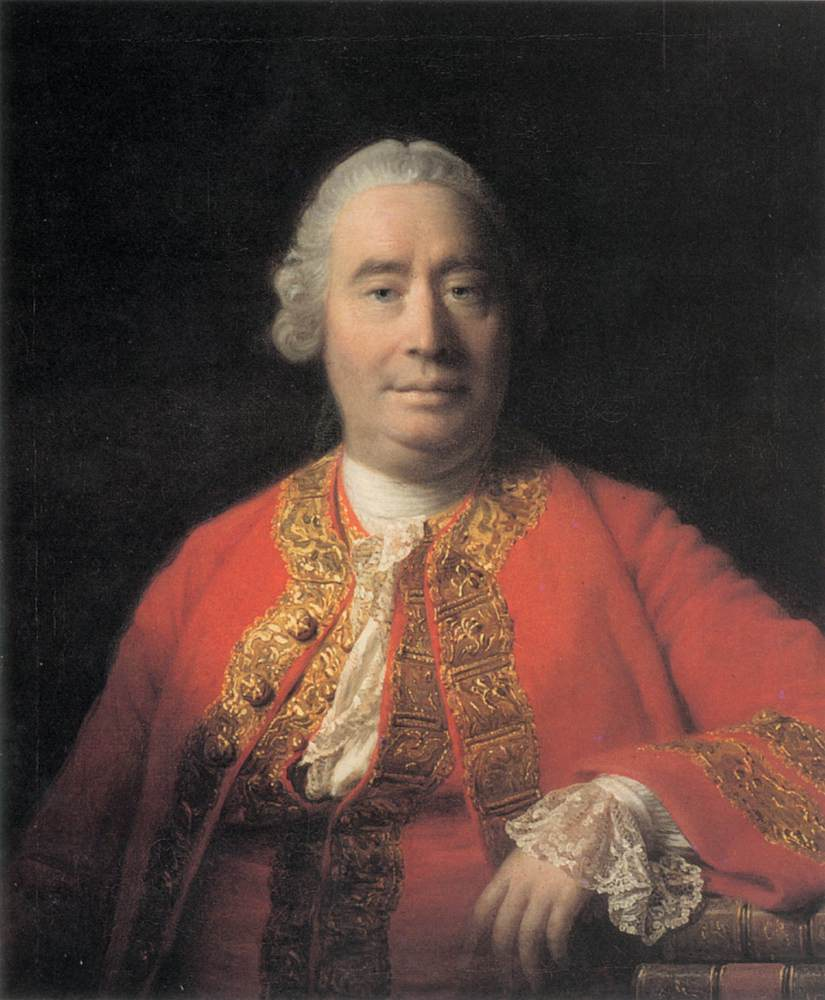
\includegraphics[height=4cm]{../../../graphics/hume.jpg}
            \end{column}
            \begin{column}{7cm}
                \begin{itemize}
                    \item<2-> In what does the merit of repaying a debt consist? 
                    \item<2-> Why is repaying a debt the object of moral approbation?
                    \item<3-> What makes repaying a debt genuinely virtuous? 
                    \item<3-> Which repayments are the objects of moral approbation?
                \end{itemize}
            \end{column}
        \end{columns}
\end{frame}

% section the_circle (end)

\subsection{Natural Motives}\label{sec:natural_motives} % (fold)

Let’s grant, for the sake of argument, that the virtuous motive could not be the ``regard to the virtue'' of the action, a sense of duty, since this involves a vicious circularity. There must then be an independent motive, distinct from the sense of duty, for any virtuous action. What independent motive could there be for just action? Hume considers three natural affections, motives that humans in their rude and natural state would be endowed with, and rejects each:
\begin{itemize}
    \item Self-love
    \item Public benevolence
    \item Private benevolence
\end{itemize}

\emph{Self-love} is a natural concern for one’s own interests. Self-love could not be the motive to just action. While there is nothing inherently wrong with acting from self-love, this passion, if unchecked, is the source of injustice. Thus, for example, if a person steals to further his own interests, he acts unjustly even though he acts from self-love.

\emph{Public benevolence} is a natural concern for the public interest. Public benevolence could not be the motive to just action. Hume gives three reasons. First, as Hume will endeavor to show, while observing the rules of justice is related to public interest, this relation is indirect and artificial---it is the general scheme established by human convention and not any particular observance of that scheme that benefits the public. A particular observance of the conventions of justice can be contrary to the public good even though the existence of the convention tends overall to increase the public good. Thus, justice may require to repay a debt to a scoundrel who will use these funds in a manner contrary to the public interest. Second, an action can be just even though it is carried out in secret. If the public can take no interest in actions it has no knowledge of, then it cannot be for the sake of public interest that the person is moved to act justly in this instance. Third, while public benevolence can motivate a person to act, this motive is too weak to explain the widespread observance of the rules of justice.

\emph{Private benevolence} is a natural concern for the interests of another. Private benevolence could not be the motive to just action. A person can be motivated to act justly even though they feel no benevolence towards the party concerned. Thus for example, a person lacks any concern for the interests of his enemy and yet can be motivated to repay a debt owed to that enemy. At least in this instance, the motive to act justly could not be private benevolence. \change

% \textbf{See Figure~\ref{fig:slide5}.}
% 
% \begin{figure}[ht]
%     \begin{center}
%         \includeslide[height=5cm]{slide5<1>}
%     \end{center}
%     \caption{Natural Motives}
%     \label{fig:slide5}
% \end{figure}

\begin{frame}<presentation>[label=slide5]
    \frametitle{Natural Motives}
        \begin{columns}
            \begin{column}{3cm}
                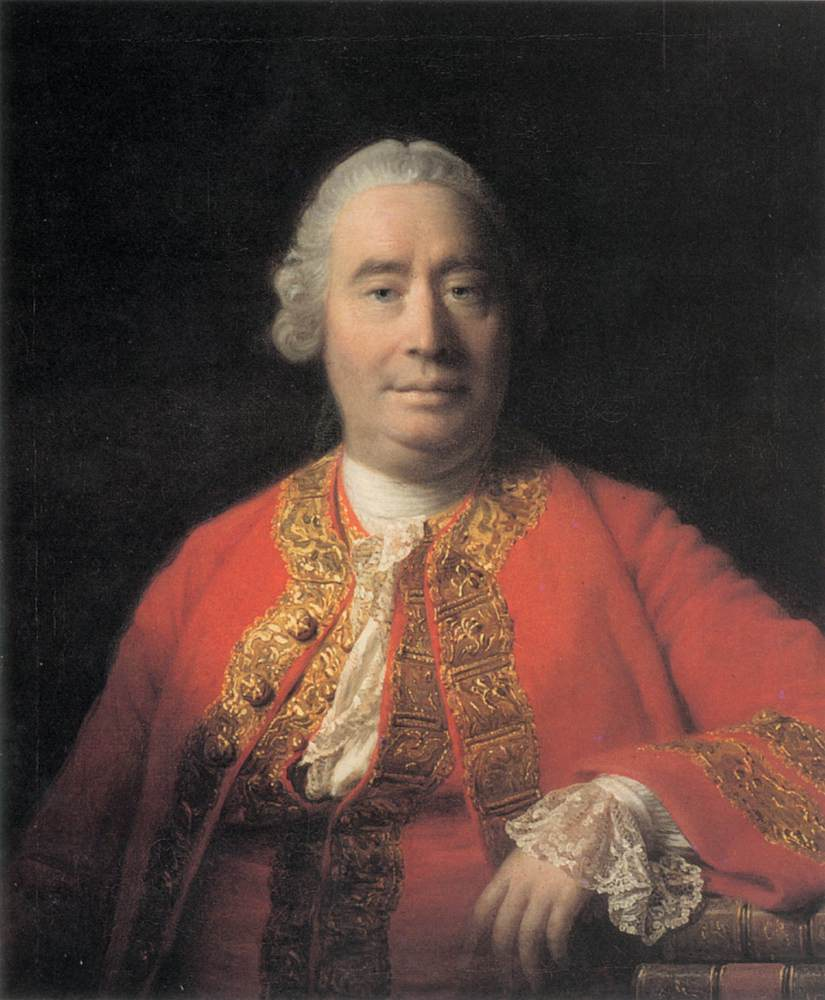
\includegraphics[height=4cm]{../../../graphics/hume.jpg}
            \end{column}
            \begin{column}{7cm}
                \begin{itemize}
                    \item Self-love
                    \item Public benevolence
                    \item Private benevolence
                \end{itemize}
            \end{column}
        \end{columns}
\end{frame}

% section natural_motives (end)

\subsection{The Final Transition}\label{sec:the_final_transition} % (fold)

Hume concludes his argument that justice is an artificial virtue as follows:
\begin{quote}
    From all this it follows, that we naturally have no real or universal motive for observing the laws of equity, but the very equity and merit of that observance; and as no action can be equitable or meritorious, where it cannot arise form some separate motive, there is here an evident sophistry and reasoning in a circle. Unless, therefore, we will allow, that nature has establish’d a sophistry, and render’d it necessary and unavoidable, we must allow, that the sense of justice and injustice is not deriv’d from nature, but arises artificially, tho’ necessarily from education, and human conventions. (\emph{Treatise}, 3.2.1.17)
\end{quote}

Hume’s reasoning is difficult to interpret here. If nature could not establish a sophistry how could human artifice? Let me speculate about how Hume might be interpreted.

First, notice that, with respect to the natural virtues, the motive to virtuous action is what bestows merit upon that action. Consider kindness to children. When you feed a hungry child, the motive is kindness, and it is the amiableness of this action, its being motivated by kindness, that bestows merit upon the action and makes it the object of moral approbation. So: 
\begin{enumerate}
    \item naturally virtuous actions have merit and are the object of moral approbation insofar as they are motivated in the relevant way, and 
    \item it is their being so motivated that bestows merit upon them and makes them the object of approbation.
\end{enumerate}


If justice were a natural virtue, then, (1) just actions would have merit and be the object of moral approbation insofar as they are motivated in the relevant way, and (2) it is their being so motivated that would bestow merit upon them and make them the object of approbation. However, just actions do not satisfy these two conditions. What could the relevant motive be? While a regard to the justice of the action can motivate a person in a civilized state to act justly, it could not bestow merit upon that action. Moreover, no independently specified natural motive, such as self-love and public and private benevolence, could be the motive to just action. Since justice does not satisfy these two conditions, justice could not be a natural virtue.

While a regard to the justice of the action might be an answer to the question, ``What makes an action genuinely just?'', it could not also be an answer to the question, ``What bestows merit upon just action and make it the object of moral approbation?'' Earlier, I worried that the alleged incoherence in reasoning in a circle turned on the supposition that these distinct questions admit of a single answer. It can seem as if either (1) Hume has confused these distinct questions or (2) that in overlooking their distinctness, Hume has failed to notice an undischarged assumption in his argument, that the motive that produces the virtuous action must also bestow merit upon it. On the present interpretation, Hume is guilty of neither. It is the assumption that justice is a natural virtue, assumed for the sake of reductio, that commits one to the claim that these two questions admit of a single answer. \change

% \textbf{See Figure~\ref{fig:slide6}.}
% 
% \begin{figure}[ht]
%     \begin{center}
%         \includeslide[height=5cm]{slide6<1>}
%     \end{center}
%     \caption{A Possible Resolution?}
%     \label{fig:slide6}
% \end{figure}

\begin{frame}<presentation>[label=slide6]
    \frametitle{A Possible Resolution?}
        \begin{columns}
            \begin{column}{3cm}
                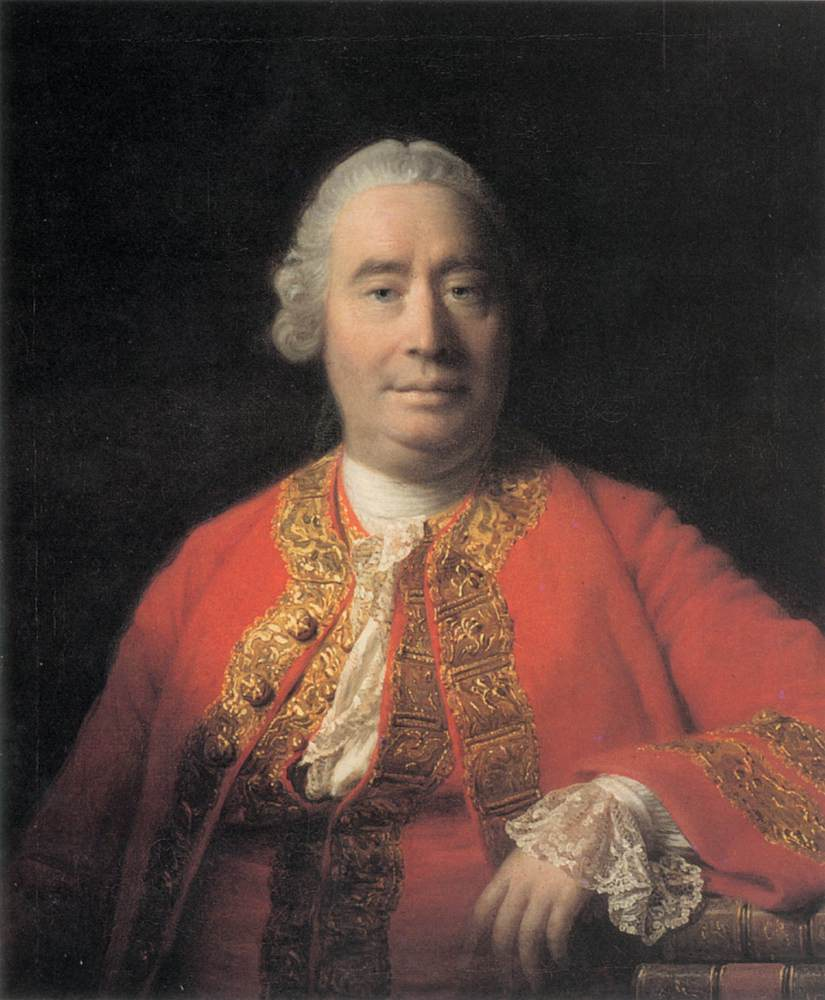
\includegraphics[height=4cm]{../../../graphics/hume.jpg}
            \end{column}
            \begin{column}{7cm}
                If justice were a natural virtue, then:
                    \begin{enumerate}
                        \item just actions would have merit and be the object of moral approbation insofar as they are motivated in the relevant way
                        \item it is their being so motivated that would bestow merit upon them and make them the object of approbation
                    \end{enumerate}
                Hume is neither guilty of a conflation, nor is making an undischarged assumption, rather he is assuming for the sake of the \emph{reductio} that justice is a natural virtue.
            \end{column}
        \end{columns}
\end{frame}

% section the_final_transition (end)

\section{Next Time}\label{sec:next_time} % (fold)

% \textbf{See Figure~\ref{fig:slide7}.}
% 
% \begin{figure}[ht]
%     \begin{center}
%         \includeslide[height=5cm]{slide7<1>}
%     \end{center}
%     \caption{Readings for Next Time}
%     \label{fig:slide7}
% \end{figure}

\begin{frame}<presentation>[label=slide7]
    \frametitle{Readings for Next Time}
        Required:
            \begin{itemize}
                \item \emph{Treatise} 3.2.2
            \end{itemize}
\end{frame}

% section next_time (end)

\end{document}
